\documentclass{standalone}

\usepackage{tikz}
\usetikzlibrary{intersections}
\usepackage{siunitx}


\usepackage{txfonts}

\begin{document}

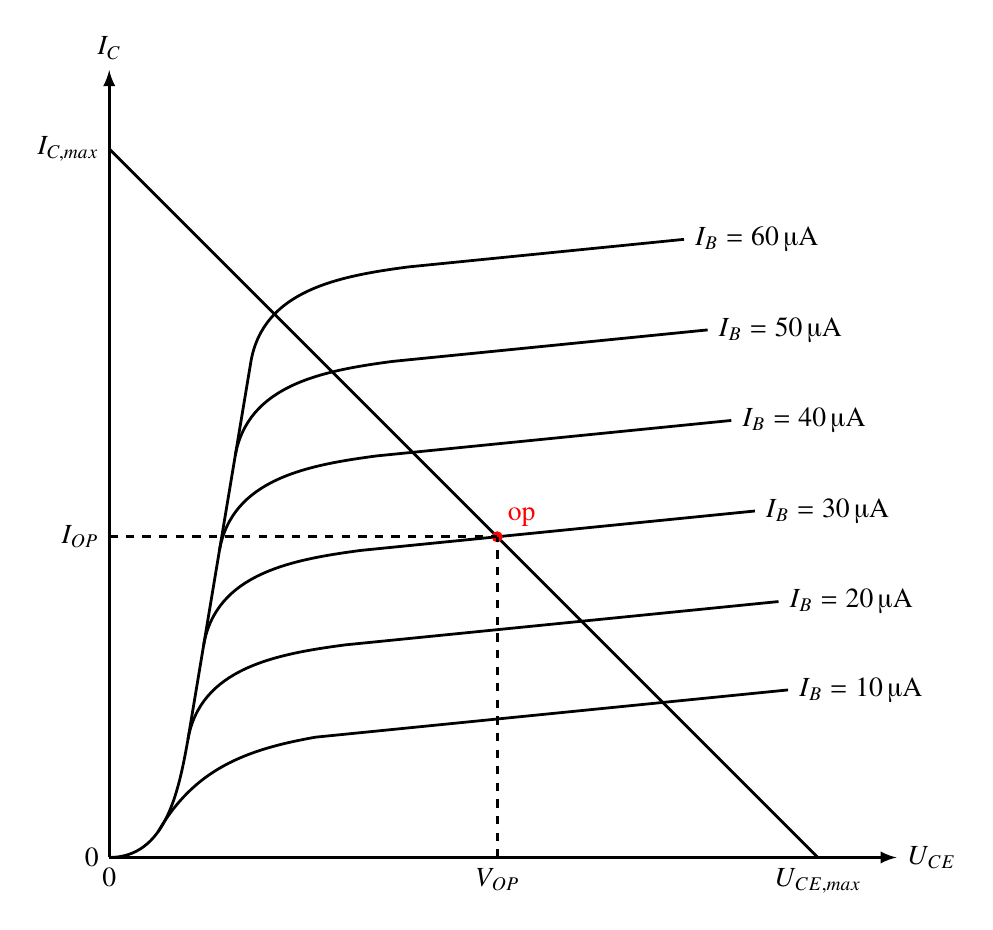
\begin{tikzpicture}[line width=1pt]

% Draw axis
\draw[-latex] node[below] {$0$} (0,0) -- (10,0) node[right] {$U_{CE}$};
\draw[-latex] node[left] {$0$} (0,0) -- (0,10) node[above] {$I_C$};

% Draw curve for Ib = 60 uA, set coordinates for other curves
\draw (0,0) to [out=0, in=260] coordinate [pos=0.4] (F) (1,1.5) coordinate (A) -- ++(0.2,1.2) coordinate (B) -- ++(0.2,1.2) coordinate(C) -- ++(0.2,1.2) coordinate (D) -- ++(0.2,1.2) to [out=80, in=187.5] ++(2,1.2) -- ++(3.5,0.35) node[right] {$I_B=\SI{60}{\micro\ampere}$};

% Draw the other curves
\draw (A) to [out=80, in=187.5] ++(2,1.2) -- ++(5.5,0.55) node[right] {$I_B=\SI{20}{\micro\ampere}$};
\draw[name path=l] (B) to [out=80, in=187.5] ++(2,1.2) -- ++(5,0.5) node[right] {$I_B=\SI{30}{\micro\ampere}$};
\draw (C) to [out=80, in=187.5] ++(2,1.2) -- ++(4.5,0.45) node[right] {$I_B=\SI{40}{\micro\ampere}$};
\draw (D) to [out=80, in=187.5] ++(2,1.2) -- ++(4,0.4) node[right] {$I_B=\SI{50}{\micro\ampere}$};
\draw (F) to [out=60, in=190] ++(2,1.2) -- ++(6,0.6) node[right] {$I_B=\SI{10}{\micro\ampere}$};;

% Draw load line
\draw[name path=k] (0,9) node[left] {$I_{C,max}$} -- (9,0) node[below] {$U_{CE,max}$};

% Find intersection of curve Ib = 30 uA and load line, name it op
\fill[red,name intersections={of=k and l, by=op}] (op) circle (2pt) node[above right] {op};

% Draw lines to Ic and Uce
\draw [dashed] ({{0,0}} |- op) node[left] {$I_{OP}$} -- (op);
\draw [dashed] ({{0,0}} -| op) node[below] {$V_{OP}$} -- (op);

\end{tikzpicture}

\end{document}
